\documentclass[12pt]{beamer}



\usepackage[utf8]{inputenc} 
\usepackage[T1]{fontenc}      
\usepackage[english]{babel} 
%\DecimalMathComma
%\usepackage[top=2cm, bottom=2cm, left=1cm, right=1cm]{geometry}

% maths packages
\usepackage{amsmath}
\usepackage{amsfonts}
\usepackage{amssymb}
%\usepackage{mhsetup}
%\usepackage{mathtools}
\usepackage{mathrsfs}
\usepackage{amsthm}
\usepackage{yhmath}
\usepackage{stmaryrd}
\PassOptionsToPackage{all}{stmaryrd}
\usepackage{graphicx}
\usepackage{sistyle}
\usepackage[version=3]{mhchem}
\usepackage{asymptote}
\usepackage{bigints}
%\usepackage[hidelinks]{hyperref}
\usepackage{centernot}
%\usepackage{dsfont}
\usepackage{bbm}
\usepackage{esint}
\usepackage{enumerate}


\SIdecimalsign{,}
\SIthousandsep{} 

%racoourci pour certain symbole

\renewcommand{\le}{\leqslant}
\renewcommand{\ge}{\geqslant}

%joli ensemble vide
\let\oldemptyset\emptyset
\let\emptyset\varnothing

% flèche d'implication qui s'adapte en largeur au texte au dessus.

\makeatletter
\newcommand*{\newextarrow}[3] {%
   \newcommand*{#1}[2][]{\ext@arrow #2{\arrowfill@#3}{##1}{##2}}
}



%\newcommand{\xRightarrow}[2][]{\ext@arrow 0359\Rightarrowfill@{#1}{#2}}
\makeatother

\newextarrow{\xRightarrow}{0959}{\Relbar\Relbar\Rightarrow}
\newextarrow{\xhookrightarrow}{99{15}{15}}{{\lhook\joinrel\relbar}\relbar\rightarrow}
\newextarrow{\xtwoheadrightarrow}{9{15}{15}{15}}{\relbar\relbar \twoheadrightarrow}
\newextarrow{\xtwoheadhookrightarrow}{9{15}{15}{15}}{{\lhook\joinrel\relbar}\relbar\twoheadrightarrow}


%symbole avec du texte au dessus ou en dessous
\newcommand{\eqat}[1]{\,\mathop{=}\limits_{#1}\,}
\newcommand{\simat}[2][]{\,\mathop{\sim}\limits_{#2}^{#1}\,}
\newcommand{\toat}[2][]{\xrightarrow[#2]{#1}}
\newcommand{\impwith}[1]{\xRightarrow[]{#1}}
\renewcommand{\O}[1][]{\underset{#1}{\mathrm{O}}}
\renewcommand{\o}[1][]{\underset{#1}{\mathrm{o}}}

%displaystyle en raccourci :
\newcommand{\ds}[1]{\displaystyle #1}
\newcommand{\dsfrac}[2]{\dfrac{\ds{#1}}{\ds{#2}}}

% mot clés en environement mathématique (et et ou sont des opératuer de logique contrairement aux autres) :
\newcommand{\et}{\;\mathrel{\mathrm{et}}\;}
%\newcommand{\et}{\mathrel{\mathrm{et}}
\newcommand{\ou}{\;\mathrel{\mathrm{ou}}\;}
\newcommand{\car}{\text{ car }} 
\newcommand{\si}{\text{ si }}
\newcommand{\av}{\text{ avec }}
\newcommand{\on}{\text{ on a : }}

\newcommand{\tq}{\mathrel{|}}% tel que avec un espacement adapté
\newcommand{\com}{,\;}

%fonction math
\newcommand{\sh}{\qopname\relax o{sh}}
\newcommand{\ch}{\qopname\relax o{ch}}
\renewcommand{\th}{\qopname\relax o{th}}
\newcommand{\ash}{\qopname\relax o{arcsh}}
\newcommand{\ach}{\qopname\relax o{arcch}}
\newcommand{\sinc}{\qopname\relax o{sinc}}
\renewcommand{\Re}{\qopname\relax o{Re}}
\renewcommand{\Im}{\qopname\relax o{Im}}
\newcommand{\Ker}{\qopname\relax o{Ker}}
\newcommand{\Vect}{\qopname\relax o{Vect}}
\newcommand{\fun}{\qopname\relax o{\mathcal{F}}}%ensemble des fonctions
\newcommand{\cont}{\qopname\relax o{\mathscr{C}}}%ensemble des fonctions continue
\newcommand{\lin}{\qopname\relax o{\mathcal{L}}}%ensemble des applications linéaire
\renewcommand{\L}{\qopname\relax o{\mathrm{L}}}%ensemble des applications itégrable
\newcommand{\Lr}{\qopname\relax o{\mathcal L}}%ensemble des applications itégrable
\newcommand{\Mat}{\qopname\relax o{\mathcal{M}}}%ensemble des matrices
\newcommand{\Tr}{\qopname\relax o{Tr}}%trace
\newcommand{\Com}{\qopname\relax o{Com}}%co-matrice

\newcommand{\pde}{{\qopname\relax o{\mathcal{P}}}}% partie de
\newcommand{\rg}{\qopname\relax o{rg}}%rang
\newcommand{\Id}{\qopname\relax o{Id}}
\newcommand{\gr}{\qopname\relax o{gr}}%groupe engendré
\newcommand{\val}{\qopname\relax o{val}}
\newcommand{\toMat}{\qopname\relax o{Mat}}
\renewcommand{\t}{{\,{}^t\!}}
\newcommand{\ki}{\qopname\relax o{\raisebox{0.5ex}{$\chi$}}}
\newcommand{\Conv}{\qopname\relax o{Conv}}%  enveloppe convexeS
\newcommand{\esp}{\qopname\relax o{E}}
\newcommand{\var}{\qopname\relax o{V}}
\renewcommand{\Pr}{\qopname\relax o{P}}
\newcommand{\cov}{\qopname\relax o{Cov}}
\newcommand{\Bij}{\qopname\relax o{Bij}}%ensemble des Bijections
\newcommand{\Aut}{\qopname\relax o{Aut}}%ensemble des Automorphismes
\newcommand{\Inn}{\qopname\relax o{Inn}}%ensemble des Automorphismes Intérieurs


% ici pour choisir entre le cardinal "Card" et le cardinal "#"
%\newcommand{\card}{\qopname\relax o{Card}} 
\newcommand{\card}{\mathopen {\mbox{\raisebox{0.1ex}{\#\!}}}}



%racourci matrice
\newcommand{\stack}[1]{\begin{matrix}#1\end{matrix}}
\newcommand{\mat}[1]{\begin{pmatrix}#1\end{pmatrix}}
\newcommand{\mdet}[1]{\begin{vmatrix}#1\end{vmatrix}}
\newcommand{\comb}[2]{\mat{#1\\#2}}


% vecteurs
\newcommand{\bvec}[1]{\overrightarrow{#1}}
\newcommand{\vvv}{|\!|\!|}

%complexes physique
\newcommand{\co}[1]{\underline{#1}}
\newcommand{\cv}[1]{\vec {\co #1}}

%opérateurs vectoriels
\newcommand{\grad}{\qopname\relax o{\bvec{\mathrm{grad}}}}
\newcommand{\rot}{\qopname\relax o{\bvec{\mathrm{rot}}}}
\newcommand{\Rot}{\qopname\relax o{Rot}}
\let\pdiv\div
\renewcommand{\div}{\qopname\relax o{div}}

%fonction physique
\newcommand{\nox}{\qopname\relax o{no}}

%crochet dans les intervalle d'entiers:
\newcommand{\ldb}{\llbracket}
\newcommand{\rdb}{\rrbracket}

%raccourci pour la logique

\newcommand{\imp}{\;\Rightarrow\;}
\newcommand{\nimp}{\;\nRightarrow\;}
\newcommand{\eq}{\;\Leftrightarrow\;}
\newcommand{\beq}{\Leftrightarrow\;}
\newcommand{\noteq}{\;\nLeftrightarrow\;}



%grands ensembles
\newcommand{\R}{\ensuremath{\mathbb{R}}}
\newcommand{\Rb}{\ensuremath{\overline{\mathbb{R}}}}
\newcommand{\N}{\ensuremath{\mathbb{N}}}
\newcommand{\Q}{\ensuremath{\mathbb{Q}}}
\newcommand{\Z}{\ensuremath{\mathbb{Z}}}
\newcommand{\C}{\ensuremath{\mathbb{C}}}
\newcommand{\U}{\ensuremath{\mathbb{U}}}
\newcommand{\ind}[1]{\mathbbm{1}_{\!#1}}


% pi sur deux et modulo 2 pi
\newcommand{\gpide}{\dfrac{\pi}{2}}
\newcommand{\pide}{\frac{\pi}{2}}
\newcommand{\ppide}{\tfrac{\pi}{2}}
\newcommand{\mdp}{[2\pi]}


%encadré aligné dans un environement align : 
%\alignedbox{partie avant le égal}{= partie après le égal}

\newlength\dlf 
\newcommand\alignedbox[2]{
&  % Alignment sign of the line
	{
	\settowidth\dlf{$\displaystyle #1$}  
	    % The width of \dlf is the width of the lhs, with a displaystyle font
	\addtolength\dlf{\fboxsep+\fboxrule}  
	    % Add to it the distance to the box, and the width of the line of the box
	\hspace{-\dlf}  
	    % Move everything dlf units to the left, so that & #1 #2 is aligned under #1 & #2
	\boxed{#1 #2}
	    % Put a box around lhs and rhs
	}
}

%Opérateurs : 
%\bsum{taille)}


\newcommand{\gcup}{ \mathop {\mbox{ $\ds\bigcup$\scalebox{1.0}[1.3]{$\uparrow$}}} }
\newcommand{\gcap}{ \mathop {\mbox{ $\ds\bigcap$\scalebox{1.0}[1.3]{$\downarrow$}}} }
\newcommand{\bigger}[2]{\mathop {\mbox{\scalebox{#2}{$\ds#1$}}}\limits}

\newcommand{\bsum}[1]{\mathop {\mbox{\scalebox{#1}{$\ds{\sum}$}}}\limits}
% pointillé mieux

\newcommand{\dddots}{\mbox{\scalebox{0.85}[1.15]{$\ddots$}}}

%définition d'application
\newcommand{\app}[2][0cm]{\hspace{-#1} \mbox{\raisebox{- \height+2ex}{$\begin{aligned}#2
\end{aligned}$}} }
\newcommand{\capp}[2][0cm]{\hspace{-#1} \mbox{\raisebox{- \height+2ex}{$\left [\begin{aligned}#2
\end{aligned}\right ]$}} }


\usepackage{tikz}

%Put a nice theme
\usetheme{Berkeley}

\title{The Blockchain technology through the bitcoin example}
\author{Luc Chabassier \and Thibaut Pérami}
\institute{École Normale Supérieure}

\begin{document}

\begin{frame}
\frametitle{Bitcoin value from start}
 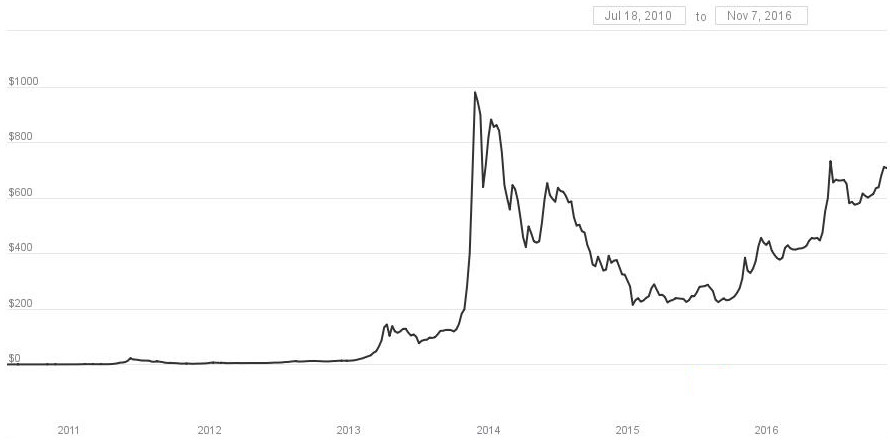
\includegraphics[scale =0.3]{FirstImage.jpeg}

\end{frame}

\begin{frame}
    \maketitle
\end{frame}

\begin{frame}
In a world more and more connected, We all do our transactions by internet and we store money in electronic banks. Notary are also entrusted with contract.

By do doing so we trust a third party and its central server which be corrupted:
\begin{itemize}
 \item on human side (investing your money in some unsafe place)
 \item or on computer side (being hacked by other people)
 \end{itemize}

\

How to ensure the inviolability of data without trusting a $3^{\mathrm {rd}}$ party ?

\end{frame}

\begin{frame}

\tableofcontents

\end{frame}

\section{Authentification}

\begin{frame}
    \frametitle{Hash functions}
    \begin{columns}[T]
        \begin{column}{.48\linewidth}
            {\color{blue}\rule{\linewidth}{4pt}

            Properties}

            $\mathscr{H} : E \rightarrow \{1, \ldots n\}$

            \begin{itemize}
                \item Quick to compute
                \item Pre-image resistance: $h, \mathscr{H}(m) = h$
                \item Second pre-image resistance: $m_1$, $\mathscr{H}(m_1) = \mathscr{H}(m_2)$
                \item Collision: $\mathscr{H}(m_1) = \mathscr{H}(m_2)$
            \end{itemize}
        \end{column}
        \hfill
        \begin{column}{.48\linewidth}
            {\color{green!40!black}\rule{\linewidth}{4pt}

            Example of SHA2-512}

            \begin{itemize}
                \item $154 MiB/s$ on regular $2GHz$ computer
                \item Around $6*10^{134}$ days on a $512$ $2GHz$ cores computer for preimage attack
                \item Since 2016, collisions can be found in reasonnable time for a weakened variant
                    of SHA2-512.
            \end{itemize}
        \end{column}
    \end{columns}
\end{frame}

\begin{frame}
    \frametitle{Asymmetric Encryption}
    \begin{columns}[T]
        \begin{column}{.48\textwidth}
            {\color{blue}\rule{\linewidth}{4pt}

            Principle}
            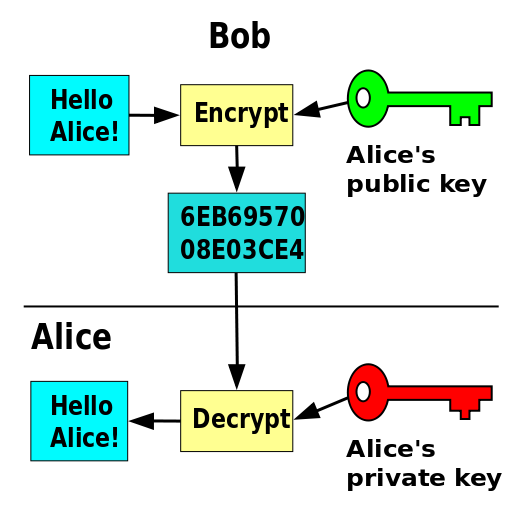
\includegraphics[width=\linewidth]{public-key.png}
        \end{column}
        \hfill
        \begin{column}{.48\linewidth}
            {\color{green!40!black}\rule{\linewidth}{4pt}

            The RSA example}

            Public key : $(n,e)$.

            Private key : $d$.

            \begin{align*}
                M & \tilde{\longrightarrow} m \\
                c &\equiv m^e (\text{mod } n) \\
                \text{Bob } & \text{sends $c$ to Alice} \\
                m' &\equiv c^d (\text{mod } n) \\
                m' = m &\tilde{\longrightarrow} M\\
            \end{align*}
        \end{column}
    \end{columns}
\end{frame}

\begin{frame}
    \frametitle{Digital signature}
    \begin{columns}[T]
        \begin{column}{.48\linewidth}
            {\color{blue}\rule{\linewidth}{4pt}

            Properties}

            \begin{itemize}
                \item Authentification
                \item Non-repudiation
                \item Integrity
            \end{itemize}
        \end{column}
        \hfill
        \begin{column}{.48\linewidth}
            {\color{green!40!black}\rule{\linewidth}{4pt}

            Implementation}

            \begin{center}
            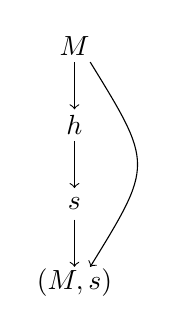
\begin{tikzpicture}
                \draw (0,0) node {$M$};
                \draw [->] (0,-0.2) -- (0,-0.8);
                \draw (0,-1) node {$h$};
                \draw [->] (0,-1.2) -- (0,-1.8);
                \draw (0,-2) node {$s$};
                \draw [->] (0,-2.2) -- (0,-2.8);
                \draw (0,-3) node {$(M,s)$};
                \draw (0.2,-0.2) .. controls (1,-1.5) .. (0.2,-2.8) [->];
            \end{tikzpicture}
            \end{center}

        \end{column}
    \end{columns}
\end{frame}

\section{Blockchain}

%ideas :
% block depencis
% network node : majority rule
% difficulty


\begin{frame}
\frametitle{Certification by sharing}
\begin{center}
\vspace{-3mm}
\begin{columns}[T]
        \begin{column}{.48\textwidth}
            {\color{blue}\rule{\linewidth}{4pt}

            Third party way}
            \begin{itemize}
            \item You and the seller go the bank and agree on terms.
            \item The bank verify and record the contract
            \item You trust the bank for keeping contract unmodified
            \end{itemize}
            
            {\color{red} Problem :}
            
            Do you really trust the bank ?

        \end{column}
        \hfill
        \begin{column}{.48\linewidth}
            {\color{green!40!black}\rule{\linewidth}{4pt}

            Peer to peer way}
            
            \begin{itemize}
            \item You tell everybody about the contract
            \item Each node verify and record it if valid
            \item You trust the majority for keeping contract unmodified
            \end{itemize}           
            
            {\color{red} Problem :}
            
            It is really easy to create many fake identity and there are multiple versions

        \end{column}
    \end{columns}

\end{center}

\end{frame}

\begin{frame}[fragile] % fragile <= asy
\frametitle{The Blockchain}
\begin{center}
\begin{asy}
unitsize(1cm);

void drawrect(string s ="", pair ori,pair size)
{
	draw(ori--(ori + (size.x,0))--(ori + size)--(ori + (0,size.y)) --cycle);
	label(s,ori + size/2);
}

drawrect((0,0),(4,2.5));
label ("Block", (2,2.15));
drawrect("Hash",(0.2,1.1),(1.7,0.7));
drawrect("Nonce",(2.1,1.1),(1.7,0.7));
drawrect("DATA",(0.2,0.2),(3.6,0.7));
draw((-0.5,1.45)--(0.2,1.45),EndArrow(SimpleHead));


drawrect((5,0),(4,2.5));
label ("Block", (7,2.15));
drawrect("Hash",(5.2,1.1),(1.7,0.7));
drawrect("Nonce",(7.1,1.1),(1.7,0.7));
drawrect("DATA",(5.2,0.2),(3.6,0.7));

draw((4,1.25)--(5.2,1.45),EndArrow(SimpleHead));

\end{asy}
\end{center}

\begin{center}
A simple rule : Always choose the longest chain
\begin{columns}[T]
        \begin{column}{.48\textwidth}
            {\color{blue}\rule{\linewidth}{4pt}
            One version}
            
			Every node agree on the longest chain: it is costly to have forgery longer than original
            

        \end{column}
        \hfill
        \begin{column}{.48\linewidth}
            {\color{green!40!black}\rule{\linewidth}{4pt}
            CPU Time Majority}
            
            Finding the right nonce is random: the one which tries more times succeed


        \end{column}
    \end{columns}

\end{center}

\end{frame}


\begin{frame}
\frametitle{Why it can't fail ?}
$p$ the probability of adding a honest block and $q = (1-p)$ the probability the attacker get a false block
\begin{itemize}
\item if $q < p$ :
\begin{itemize}
\item reduce gap by one: $\frac{q}{p}$
\item reduce gap by $n$: $\left (\frac{q}{p}\right )^n$
\end{itemize}
\item if $p \ge q$ it is certain that the adversary will win : 
\end{itemize}
\begin{center}
\color{red!50!black} \large The attack of the $51\%$
\end{center}

In practice: $10^{18}$ operations by second in current network.

\end{frame}

\section{Applications}

\begin{frame}
    \frametitle{Applications}
    \begin{itemize}
        \item Crypto-currencies
        \item Smart contracts
        \item Proof of existence
        \item Proof of possession
        \item Online voting
        \item And so much more \ldots
    \end{itemize}
\end{frame}

\begin{frame}
\frametitle{Conclusion}
\begin{columns}[T]
        \begin{column}{.48\textwidth}
            {\color{blue}\rule{\linewidth}{4pt}
            Advantages}
            Secure and reliable way to
            store data in a chronological order.

            Many revolutionary applications.
        \end{column}
        \hfill
        \begin{column}{.48\linewidth}
            {\color{green!40!black}\rule{\linewidth}{4pt}
            Limits}
            Waste of computing power: the bitcoin network
            is powerfull enough to simulate a human brain synapse by synapse, and
            consumes (as of 2015) $1.46$ terawatt-hour per year, enough to supply
            135000 american homes for a year in electricity.
        \end{column}
    \end{columns}
\end{frame}

\begin{frame}
\frametitle{Bibliography}
\begin{itemize}
\item Original article from Satoshi Nakamoto at https://bitcoin.org/bitcoin.pdf
\item Article on Quartz newspaper : http://qz.com/84056/the-bitcoin-network-is-now-more-powerful-than-the-top-500-supercomputers-combined/
\item Real time chart: http://www.coindesk.com/price/
\item Article on Inverse : https://www.inverse.com/article/6994-bitcoin-paves-the-way
\end{itemize}

\end{frame}

\begin{frame}

Are you ready to trust all your money and engagement to a peer-to-peer blockchain or do you need the feeling of security a bank give to you ?


\end{frame}

\end{document}
